% !TeX program = lualatex
% !TeX encoding = utf8
% !TeX spellcheck = uk_UA
% !BIB program = biber


\documentclass{LabBook}
\addbibresource{\jobname.bib}
%\usepackage{caption}


%========================================================================================================
%
%									      Вихідні дані докумета
%
%========================================================================================================

\title{Електрика та магнетизм}
\def\subtitle{Лабораторний практикум. Змінний струм}

\newcommand{\inX}{%
\tikz[baseline=-0.3em]{\draw (165:0.5em) arc (165:-165:0.5em); \draw[-latex] (-0.8em,0) -- ++(1em,0);} X%
}

%========================================================================================================
%
\input{CoverPage}%					      Титульна сторінка
%
%========================================================================================================
\date{}

\begin{document}
\CoverPage
\maketitle
\makeinfopage
\tableofcontents
\thispagestyle{empty}
\clearpage

%===============================================================================
%
%									      Вставка файлів розділів
%
%===============================================================================

%\setcounter{part}{1}
%\renewcommand{\thechapter}{3.\arabic{chapter}}
\newcommand{\Chapters}{
	LabRC,
	LabRL,
	LabRLC
}

%========================================================================================================
\pagestyle{theorpart}
% !TeX program = lualatex
% !TeX encoding = utf8
% !TeX spellcheck = uk_UA
% !TeX root =../LabWork.tex

\part{Теоретична частина}

\section{Означення}

Змінний струм --- електричний струм, сила та напрямок якого періодично змінюються з часом, на відміну від постійного струму, який тече лише в одному напрямку.

\noindent\bigskip%
\begin{More}

	Змінний струми називається \emph{квазістаціонарним} якщо він повільно змінюється з часом настільки, щоб забезпечити миттєві значення сили струму однаковими в усіх перерізах кола. Умова квазістаціонарності для змінного струму буде задовольнятись лише в обмеженій області простору в безпосередній близькості від генератора змінної напруги, для якої виконується умова $\tau = l/c \ll T$, де $\tau$~--- час поширення електромагнітного поля вздовж кола, $l$~--- характерні розміри електричного кола, $c$~--- швидкість поширення електромагнітної хвилі, $T$~--- період коливань генератора, іншими словами, умова квазістаціонарності задовольняється, якщо розміри кола значно менші за довжину електромагнітної хвилі $l \ll cT$. В такому випадку, для миттєвих значень квазістаціонарних струмів виконуються закон Ома і правила Кірхгофа.

	Надалі, під змінним струмом мається на увазі саме квазістаціонарний змінний струм.

\end{More}

Звичайним виглядом кривої змінного струму в більшості електричних кіл живлення є синусоїда, верхній півперіод якої відповідає додатному напрямку струму, а нижній~--- від'ємному, такий струм називається синусоїдальним (рис.~\ref{plt:sinusoidal_current}). Синусоїдальний струм --- елементарний, тобто його неможливо розкласти на інші більш прості змінні струми. Основними характеристиками такого струму є амплітуда, частота та зсув фаз між струмом та напругою на генераторі.

\begin{center}
    % !TeX program = lualatex
% !TeX encoding = utf8
% !TeX spellcheck = uk_UA
% !TeX root =../LabWork.tex

	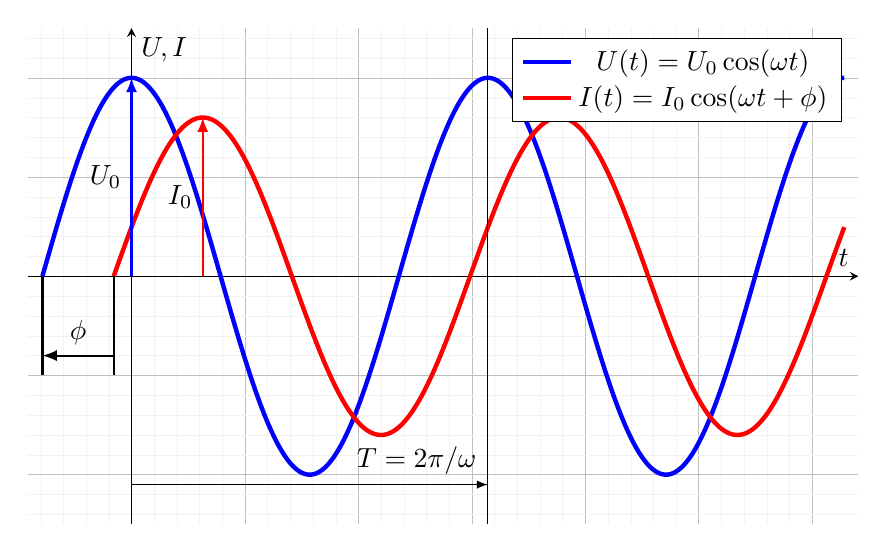
\begin{tikzpicture}
		\begin{axis}[%
				grid = both,
				major grid style={line width=.2pt,draw=gray!50},
				minor tick num = 4,
				minor grid style = {line width=.1pt,draw=gray!10},
				axis lines = middle,
				axis line style={-stealth},
				xlabel={$t$},
				ylabel={$U,I$},
				ytick style={draw=none},
				xtick style={draw=none},
				xticklabels={},yticklabels={},
				xmin = -pi/2,
				xmax = 4*pi,
				ymin = -1,
				ymax =  1,
				width=1\linewidth,
				height=0.65\linewidth,
				enlargelimits={abs=0.25},
			]
			\addplot+[ultra thick, samples=1000, blue, no marks, domain={-pi/2:4*pi}] {cos(deg(x))};
			\addplot+[ultra thick, samples=1000, red, no marks, domain={-(pi/2-0.4*pi):4*pi}] {4/5*cos(deg(x - 0.4*pi))};
			\draw[-latex, blue, thick] (axis cs:0,0) -- node[left, color = black] {$U_0$} (axis cs:0,1);
			\draw[-latex, red, thick] (axis cs:0.4*pi,0) -- node[left, color = black] {$I_0$} (axis cs:0.4*pi,4/5);
			\draw[thick] (axis cs:-pi/2,0) -- (axis cs:-pi/2,-0.5) (axis cs:-pi/2+0.4*pi,0) -- (axis cs:-pi/2+0.4*pi,-0.5);
			\draw[thick, latex-] (axis cs: -pi/2,-0.4) -- node[above] {$\phi$} (axis cs:-pi/2+0.4*pi,-0.4);
			\draw[] (axis cs: 2*pi,-1.25) -- (axis cs: 2*pi,1.25);
			\draw[-latex] (axis cs: 0,-1.05) -- node[above, pos=0.8] {$T = 2\pi/\omega$} (axis cs:2*pi,-1.05);
			\legend{$U(t) = U_0\cos(\omega t )$, $I(t) = I_0\cos(\omega t + \phi)$}
		\end{axis}
	\end{tikzpicture}
	\captionof{figure}{Графічне зображення синусоїдального змінного струму}
	\label{plt:sinusoidal_current}
\end{center}

\section{Діючі значення сили струму та напруги}

Окрім зазначених характеристик, змінний струм також характеризують діючим значенням $I_{\eff}$. \emph{Діюче значення змінного струму дорівнює такому значенню постійного струму, який за час, що дорівнює періоду виділяє на тому ж активному опорі таку ж кількість теплоти, що і даний змінний струм.}

Згідно закону Джоуля-Ленца, постійний струм величиною $I_{\eff}$  за час $T$ на резисторі $R$ виділить кількість теплоти $Q  = I_{\eff}^2 R T$, а змінний струм $I$ за період виділить кількість теплоти $Q = \int\limits_0^T I^2 R dt$.

Прирівнюючи ці два вирази отримаємо:
\[
	I_{\eff} = \sqrt{\frac1T\int\limits_0^T I^2 dt} = \sqrt{\left\langle I^2\right\rangle }.
\]
В цьому виразі під коренем стоїть величина, яка є середнім квадратичним значенням струму за період $T$. Для синусоїдального струму $I = I_0\cos(\omega t + \phi)$, як легко переконатись, ця величина дорівнює $\dfrac{I_0^2}{2}$, а тому, діюче значення струму дорівнюватиме:
\begin{equation}\label{Ieff}
	I_{\eff} = \frac{I_0}{\sqrt2}.
\end{equation}

Повторюючи аналогічні викладки для напруги можна отримати, вираз для діючого значення напруги:
\begin{equation}\label{Ueff}
	U_{\eff} = \frac{U_0}{\sqrt2}.
\end{equation}

Як видно з цих формул, діючі значення сили струму та напруги в $\sqrt2$ разів менше їх амплітудних значень.

\noindent\bigskip%
\begin{More}

	На шкалах вимірювальних приладів наносяться зазвичай саме діючі значення струму та напруги.

	Згідно даних, наведених в статті вікіпедії \href{https://uk.wikipedia.org/wiki/Побутова_електрична_мережа}{<<Побутова електрична мережа>>} наразі в Україні мережа має діюче значення напруги $230$~В  і частоту $50$~Гц.
\end{More}

\section{Послідовне коло змінного струму}

Будь-яке реальне електричне коло змінного струму містить активний опір (опір провідників, нагрівальних приладів, тощо), ємнісний опір (ємність провідників, конденсаторів) та індуктивний опір (обмотки електродвигунів, котушки електромагнітних приладів). Якщо до такого кола під’єднати двопроменевий осцилограф, то ми будемо спостерігати осцилограми коливань сили струму і напруги, які не збігаються за фазою (рис.~\ref{plt:sinusoidal_current}). Змінюючи індуктивність котушки (наприклад, вносячи залізне осердя) або ємність батареї конденсаторів, будемо спостерігати, що змінюється і різниця фаз.

\begin{wrapfigure}{L}{0.4\linewidth}
	\begin{tikzpicture}[every circuit symbol/.style={thick}]
		\draw[thick] (0,-2) coordinate (START) to [ac source={rotate=-90,info={left:$\mathcal{E}$}}] (0,2) -- ++(3,0) coordinate (A) to [resistor={info'={$R$}}] ++(0,-4/3) coordinate (B) to [inductor={info'={$L$}}] ++(0,-4/3) coordinate (C) to [capacitor={info'={$C$}}] ++(0,-4/3) coordinate (D)  -- (START)
		;
		\draw[red] (A) -- ++(1,0) (B) -- ++(1,0) (C) -- ++(1,0) (D) -- ++(1,0);
		\draw[<->, red] ([xshift=0.75cm]A) -- node[right, color=black] {$U_R$} ([xshift=0.75cm]B);
		\draw[<->, red] ([xshift=0.75cm]B) -- node[right, color=black] {$U_L$} ([xshift=0.75cm]C);
		\draw[<->, red] ([xshift=0.75cm]C) -- node[right, color=black] {$U_C$} ([xshift=0.75cm]D);
	\end{tikzpicture}
	\caption{Послідовне $RLC$-коло}
	\label{pic:S-RLC}
\end{wrapfigure}
Розглянемо електричне коло з активним, ємнісним та індуктивним навантаженнями, які з’єднані послідовно (рис.~\ref{pic:S-RLC}) (таке коло ще називають послідовним колом змінного струму).  З фізичної точки зору, така система є коливальним контуром, в якому здійснюватимуться вимушені гармонічні коливання під дією гармонічної напруги:
\begin{equation}\label{U_0}
	\mathcal{E} = \mathcal{E}_0\cos\omega t
\end{equation}

Згідно законів Ома, в довільний момент часу сума напруг на кожному елементі дорівнюватиме напрузі на генераторі:
\begin{equation}\label{ID_KL}
	U_R + U_L + U_C = IR + L\frac{dI}{dt} +  \frac{1}{C}\int I dt = \mathcal{E}_0\cos\omega t,
\end{equation}
де напруги на кожному елементі виражені через струм в колі, оскільки саме струм у випадку послідовного з'єднання буде однаковим на кожному елементі.

Отже, рівнянні~\eqref{ID_KL} є лінійним диференціальним рівнянням відносно сили струму. У випадку \emph{встановлених} коливань, розв'язок цього рівняння будемо шукати у вигляді:
\begin{equation}\label{I}
	I = I_0\cos(\omega t + \phi),
\end{equation}
де $I_0$~--- амплітуда струму в колі (однакова на всіх елементах), $\phi$~--- зсув фаз між напругою та струмом.


\subsection{Метод комплексних амплітуд}

Розв'яжемо рівняння~\eqref{ID_KL} і знайдемо силу струму в колі, а також напруги на кожному з елементів кола. Одним із способів його розв'язку є \emph{метод комплексних амплітуд}.

\noindent\bigskip% 
\begin{More}
	Мати справу з гармонічними функціями не так просто, набагато легше працювати з експоненційними функціями, вони зручні при інтегруванні та диференціювання. Формула Ейлера
	\begin{equation*}
		e^{i\phi} = \cos\phi + i\sin\phi,
	\end{equation*}
	є ключовим виразом, який пов'язує гармонічні функції та комплекснозначну експоненту.

	Будь-яке комплексне число вигляду $z = a + ib$ можна представити у вигляді комплексної експоненти:
	\[
		z = |z|e^{\phi},
	\]
	де величина $|z| = \sqrt{a^2 + b^2}$ --- називається модулем комплексного числа $z$, а $\phi$~--- його фазою, яка визначається як $\tg\phi = \dfrac{b}{a}$, а його дійсна частина дорівнює $\Re{(z)} =|z|\cos\phi$.
\end{More}


Суть цього методу полягає в тому, що напругу слід представити як $\hat{\mathcal{E}} = \hat{\mathcal{E}}_0e^{i\omega t}$, а розв'язок шукати у вигляді $\hat{I} = \hat{I}_0e^{i\omega t}$, де величини $\hat{U}_0$  та $\hat{I}_0$ є комплексними амплітудами (<<шляпка>> над відповідною величиною означає, що вона є комплексною). Після розрахунків, для отримання вимірюваної величини, слід взяти дійсну частину отриманого комплексного виразу, попередньо представивши його у експоненційній формі: $I = |\hat{I}_0| \Re(e^{i(\omega t + \phi)})$. Такий метод називається \emph{методом комплексних амплітуд}. Скористаємось таким методом  і знайдемо розв'язок  шляхом підстановки $\hat{I} = \hat{I}_0e^{i\omega t}$ в рівняння~\eqref{ID_KL}:
\begin{equation}\label{Complex_Amplitudes}
	\hat{I}_0 R  + \hat{I}_0 i\omega L + \hat{I}_0 \frac{1}{i\omega C} = \hat{\mathcal{E}}_0.
\end{equation}
В останньому рівнянні зручно ввести величини $\hat{X}_L = i\omega L$ та $\hat{X}_C = \frac{1}{i\omega C}$, які називаються \emph{комплексними опорами} котушки та конденсатора, відповідно.

Отже, рівняння~\eqref{Complex_Amplitudes} можна представити у вигляді  $\hat{I}_0 \hat{Z} = \hat{\mathcal{E}}_0$, де $\hat{Z}$ називається \href{http://femto.com.ua/articles/part_1/1313.html}{\emph{імпедансом}} послідовного кола і визначається формулою:
\begin{equation}\label{total_impedance}
	\hat{Z} = R + \hat{X}_L + \hat{X}_C = R  +   i\left(  \omega L - \frac{1}{\omega C} \right) .
\end{equation}

\begin{More}

	Завдяки методу комплексних амплітуд, аналіз режимів в електричних колах суттєво спрощується. Рівняння електричного стану для кола змінного струму в комплексній формі подібні до рівнянь електричного стану для кіл постійного струму. Завдяки цьому, використання комплексних опорів, комплексних амплітуд струмів і напруг дозволяє записувати закони Ома таким же чином, як і в для постійних струмів.
\end{More}

Використовуючи рівняння~\eqref{Complex_Amplitudes}, бачимо, що комплексна амплітуда струму дорівнює:
\begin{equation}\label{CI0}
	\hat{I}_0 = \frac{\hat{\mathcal{E}}_0}{R  +   i\left(  \omega L - \frac{1}{\omega C} \right)}.
\end{equation}

Виразимо останнє рівняння в експоненційній формі (позбавившись комплексності знаменника домноженням на комплексно-спряжену величину і скориставшись формулою Ейлера):
\begin{equation}\label{CI0_phase}
	\hat{I}_0 = \frac{\hat{\mathcal{E}}_0e^{i\phi}}{\sqrt{R^2  +   \left(  \omega L - \frac{1}{\omega C} \right)^2}},
\end{equation}
де $\phi$~--- є зсувом фаз між силою струму та напругою, і визначається співвідношенням
\begin{equation}\label{S-phase_shift}
	\tg\phi = \frac{\omega L - \frac{1}{\omega C}}{R},
\end{equation}
а модуль імпедансу
\begin{equation}
	Z = |\hat{Z}| = \sqrt{R^2  +   \left(  \omega L - \frac{1}{\omega C} \right)^2}.
\end{equation}
%Отже, вираз для комплексного струму буде виглядати наступним чином (пам'ятаємо, що $\hat{\mathcal{E}}_0 = U_0$):
%\begin{equation}\label{CI0}
%	\hat{I}= \frac{\mathcal{E}_0}{Z}e^{i(\omega t + \phi)},
%\end{equation}
%а його дійсна частина буде розв'язком рівняння~\eqref{ID_KL}:
%\begin{equation}
%	I= \frac{U_0}{Z}\cos(\omega t + \phi).
%\end{equation}

З урахуванням поняття імпедансу, рівняння~\eqref{Complex_Amplitudes} можна записати у вигляді
\begin{equation}\label{eq:S_sumU}
	\hat{U}_{0_R} + \hat{U}_{0_L} + \hat{U}_{0_C} = \hat{\mathcal{E}}_{0},
\end{equation}
де
\begin{equation}\label{eq:U}
	\hat{U}_{0_R} = \hat{I}_{0} R, \quad \hat{U}_{0_L} = \hat{I}_{0} \hat{X}_L, \quad \hat{U}_{0_C} = \hat{I}_{0} \hat{X}_C.
\end{equation}

%Виразимо їх в експоненційній формі:
%\begin{equation*}
%	\hat{U}_{0_R} = I_0 R,  \quad \hat{U}_{0_L} = I_0\omega Le^{i\frac{\pi}{2}}, \quad \hat{U}_{0_C} = \frac{I_0}{\omega C}e^{-i \frac{\pi}{2}}, \quad \hat{\mathcal{E}}_{0} = \mathcal{E}_0.
%\end{equation*}

\subsection{Метод векторних діаграм}

Для кращого розуміння і наочності представлення коливальних процесів, окрім методу комплексних амплітуд також використовується \emph{метод векторних діаграм}. Суть цього методу полягає в тому, що величини, які змінюються за гармонічним законом зображуються у вигляді вектора, довжина якого дорівнює амплітуді коливань і який обертається проти годинникової стрілки з кутовою швидкістю, що дорівнює частоті коливань $\omega$ навколо довільно вибраного полюса (рис.~\ref{fig:vector_diagram}). Оскільки векторна діаграма малюється, то вектори прийнято зображувати під кутом, що дорівнює $\phi$. В якості осі вибирається вектор іншої коливальної величина, а $\phi$~--- є зсувом фаз між коливальними величинами. 

%---------------------------------------------------------
\begin{figure}[h!]\centering
    \begin{tikzpicture}
            \pgfmathsetmacro{\ang}{40}
            \node[fill=black,circle,scale=0.3, pin={[pin distance=1cm]-90:{полюс}}] at (0,0)  {};
            \draw (0,0) -- ++(10,0) node[pos=0.8, below] {вісь};
            \draw[-latex, red, thick] (0,0) -- node[anchor=south east, black] {$\vec{I}_0$} (\ang:8) coordinate (END);
            \draw[dashed] (END) -- (END|-0,0);
            \path (0,0) --  node[below] {$I = I_0\sin(\omega t +\phi)$} (END|-0,0);
            \draw[->] (2,0) arc (0:\ang:2) node[pos=0.5, anchor=west] {$\phi$};
            \draw[-latex] (-120:0.5) arc (-120:120:0.5) node[pos=1, anchor=east] {$\omega$};
    \end{tikzpicture}
\caption{Представлення гармонічного коливання у вигляді вектора}
\label{fig:vector_diagram}
\end{figure}
%---------------------------------------------------------
Розглянемо деякі часткові випадки:
\begin{enumerate}
\item У коло включено лише активний опір $R$ ($C=\infty$, $L = 0$). У цьому
випадку з формул~\eqref{S-phase_shift} випливає, $\phi = 0$. Струм через опір~\eqref{CI0_phase} збігається по фазі з напругою на ньому:
\[
    \hat{I}_0 = \frac{\hat{\mathcal{E}}_{0}}{R}.
\]

Векторна діаграма має вигляд:
\begin{center}
    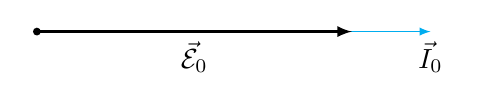
\begin{tikzpicture}
            \pgfmathsetmacro{\ang}{0}
            \node[fill=black,circle,scale=0.3, pin={[pin distance=0cm]-90:{}}] at (0,0)  {};
            \draw[-latex, cyan] (0,0) -- ++(5,0) node[pos=1, below, black] {$\vec{I}_0$};
            \draw[ultra thick, -latex, black, thick] (0,0) -- node[below, black] {$\vec{\mathcal{E}}_0$} (\ang:4) coordinate (END);
    \end{tikzpicture}
\end{center}
\item У коло увімкнена один лише конденсатор ємністю $C$ (конденсатор без втрат) ($R=0$, $L = 0$). У цьому випадку $\phi = \frac\pi2$ (струм по фазі випереджає напругу на $\frac\pi2$):
\[
    \hat{I}_0 = \omega C\hat{\mathcal{E}}_{0}e^{i\frac\pi2}.
\]
Векторна діаграма має вигляд:
\begin{center}
    \begin{tikzpicture}
            \pgfmathsetmacro{\ang}{-90}
            \node[fill=black,circle,scale=0.3, pin={[pin distance=0cm]-90:{}}] at (0,0)  {};
            \draw[-latex, cyan] (0,0) -- ++(3.5,0) node[pos=1, right, black, black] {$\vec{I}_{0}$};
            \draw[ultra thick,-latex, black, thick] (0,0) -- node[left, black] {$\vec{\mathcal{E}}_0$} (\ang:3) coordinate (END);
    \end{tikzpicture}
\end{center}
\item  У коло увімкнена лише  індуктивність  $L$ (котушка, активним опором якої при даній частоті можна знехтувати) ($C=\infty$, $R = 0$). Як випливає з ~\eqref{S-phase_shift} при-цьому $\phi = -\frac\pi2$ (струм
в колі відстає від напруги по фазі на $\frac\pi2$):
\[
    \hat{I}_0 = \frac{\hat{\mathcal{E}}_{0}e^{-i\frac\pi2}}{\omega L}.
\]
Векторна діаграма має вигляд:
\begin{center}
    \begin{tikzpicture}
            \pgfmathsetmacro{\ang}{90}
            \node[fill=black,circle,scale=0.3, pin={[pin distance=0cm]-90:{}}] at (0,0)  {};
            \draw[-latex, cyan] (0,0) -- ++(3.5,0) node[pos=1, right, black, black] {$\vec{I}_{0}$};
            \draw[ultra thick,-latex, black, thick] (0,0) -- node[left, black] {$\vec{\mathcal{E}}_0$} (\ang:3) coordinate (END);
    \end{tikzpicture}
\end{center}
\item  Послідовне $RC$-коло. В цьому випадку ($L=0$). Як випливає з ~\eqref{S-phase_shift}:
\begin{align}
    \tg\phi &= -\frac{1}{\omega RC}, \\
    \hat{I}_0 &= \frac{\hat{\mathcal{E}}_{0}e^{-i\phi}}{\sqrt{R^2 + \left( \frac{1}{\omega C}\right)^2 }}.
\end{align}
Векторна діаграма має вигляд:
\begin{center}
    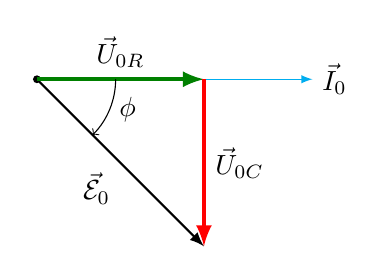
\begin{tikzpicture}
            \pgfmathsetmacro{\phase}{-45}
            \node[fill=black,circle,scale=0.3, pin={[pin distance=0cm]-90:{}}] at (0,0)  {};
            \draw[-latex, cyan] (0,0) -- ++(3.5,0) node[pos=1, right, black] {$\vec{I}_{0}$};
            \draw[-latex, black, thick] (0,0) -- node[anchor=north east, black] {$\vec{\mathcal{E}}_0$} ++(\phase:3) coordinate (PHASE);
            \draw[ultra thick,-latex,  green!50!black] (0,0) -- node[above, black] {$\vec{U}_{0R}$} (PHASE|-0,0);
            \draw[ultra thick,-latex,  red] (PHASE|-0,0) -- node[right, black] {$\vec{U}_{0C}$} (PHASE);
            \draw[->] (1,0) arc (0:\phase:1) node[pos=0.5, anchor=west] {$\phi$};
    \end{tikzpicture}
\end{center}
\item  Послідовне $RL$-коло. В цьому випадку ($C=\infty$). Як випливає з ~\eqref{S-phase_shift}:
\begin{align}
    \tg\phi &= \frac{\omega L}{R}, \\
    \hat{I}_0 &= \frac{\hat{\mathcal{E}}_{0}e^{-i\phi}}{\sqrt{R^2 + \left(\omega L\right)^2 }}.
\end{align}
Векторна діаграма має вигляд:
\begin{center}
    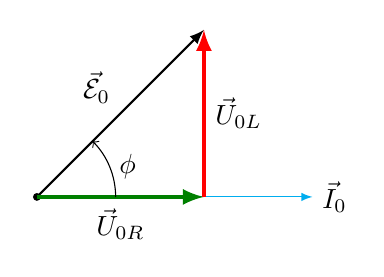
\begin{tikzpicture}
            \pgfmathsetmacro{\phase}{45}
            \node[fill=black,circle,scale=0.3, pin={[pin distance=0cm]-90:{}}] at (0,0)  {};
            \draw[-latex, cyan] (0,0) -- ++(3.5,0) node[pos=1, right, black] {$\vec{I}_{0}$};
            \draw[ultra thick,-latex, black, thick] (0,0) -- node[anchor=south east, black] {$\vec{\mathcal{E}}_0$} ++(\phase:3) coordinate (PHASE);
            \draw[ultra thick,-latex,  green!50!black] (0,0) -- node[below, black] {$\vec{U}_{0R}$} (PHASE|-0,0);
            \draw[ultra thick,-latex,  red] (PHASE|-0,0) -- node[right, black] {$\vec{U}_{0L}$} (PHASE);
            \draw[->] (1,0) arc (0:\phase:1) node[pos=0.5, anchor=west] {$\phi$};
    \end{tikzpicture}
\end{center}

\clearpage

\item  Послідовне $RLC$-коло.
%---------------------------------------------------------
\begin{figure}[h!]\centering
 % !TeX program = lualatex
% !TeX encoding = utf8
% !TeX spellcheck = uk_UA
% !TeX root =../LabWork.tex

	\begin{subfigure}[b]{0.30\linewidth}
		\centering
		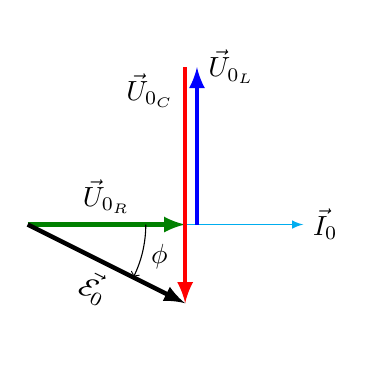
\begin{tikzpicture}[
				declare function = {
						UC = 3;
						UL = 2;
						UR = 2;
						DLC = (UL - UC);
						PhU = atan (DLC/UR);
					},
			]
			\path[use as bounding box] (0,-1.5) rectangle ++(4,4);
			\draw[-latex, cyan] (0,0) -- ++(3.5,0) node[right, color=black] {$\vec{I}_0$};
			\draw[-latex,  green!50!black,ultra thick] (0,0) -- ++(UR,0) node[above, pos=0.5, color=black] {$\vec{U}_{0_R}$};
			\draw[-latex,  blue, ultra thick] (UR+0.15,0) -- ++(0,UL) node[right, color=black] {$\vec{U}_{0_L}$};
			\draw[-latex,  red, ultra thick] (UR,UL) -- ++(0,-UC) node[left, color=black, pos=0.1] {$\vec{U}_{0_C}$};
			\draw[-latex,  black, ultra thick] (0,0) -- (PhU:{UR/cos(PhU)}) node[below, color=black, pos=0.5, sloped] {$\vec{\mathcal{E}}_{0}$} coordinate (U);
			%	\draw[dashed] (\UR,0) -- (U) (0,\DLC) -- (U);
			\draw[->] (0,0) ++(1.5,0) arc(0:PhU:1.5) node[pos=0.6, right] {$\phi$};
		\end{tikzpicture}
		\caption{$\omega < \omega_0$}
		\label{pic:S-vector_diagrams<}
	\end{subfigure}
	\begin{subfigure}[b]{0.30\linewidth}
		\centering
		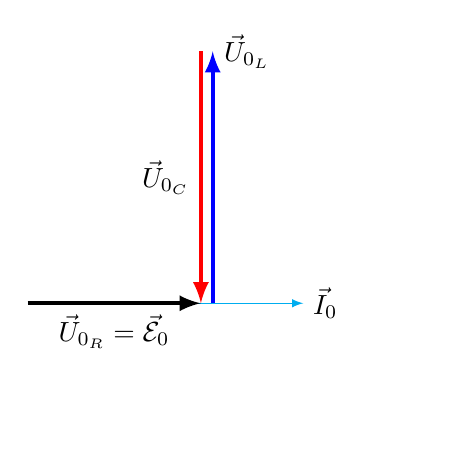
\begin{tikzpicture}[
				declare function = {
						UC = 3.2;
						UL = 3.2;
						UR = 2.2;
						DLC = (UL - UC);
						PhU = atan (DLC/UR);
					},
			]
			\path[use as bounding box] (0,-1.5) rectangle ++(5,5);
			\draw[-latex, cyan] (0,0) -- ++(3.5,0) node[right, color=black] {$\vec{I}_0$};
			\draw[-latex,  black,ultra thick] (0,0) -- ++({2/cos(atan(1/2.2)},0) node[below, pos=0.5, color=black] {$\vec{U}_{0_R} = \vec{\mathcal{E}}_{0}$};
			\draw[-latex,  blue, ultra thick] (UR+0.15,0) -- ++(0,UL) node[right, color=black] {$\vec{U}_{0_L}$};
			\draw[-latex,  red, ultra thick] (UR,UL) -- ++(0,-UC) node[left, color=black, pos=0.5] {$\vec{U}_{0_C}$};
		\end{tikzpicture}
		\caption{$\omega = \omega_0$}
		\label{pic:S-vector_diagrams=}
	\end{subfigure}
	\begin{subfigure}[b]{0.30\linewidth}
		\centering
		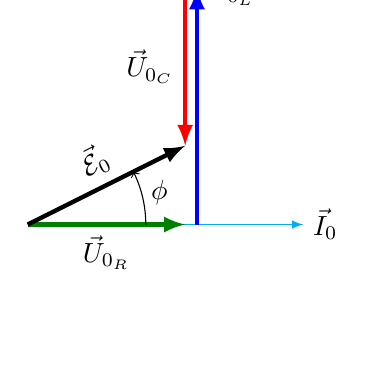
\begin{tikzpicture}[
				declare function = {
						UC = 2;
						UL = 3;
						UR = 2;
						DLC = (UL - UC);
						PhU = atan (DLC/UR);
					},
			]
			\path[use as bounding box] (0,-1.5) rectangle ++(4,4);
			\draw[-latex, cyan] (0,0) -- ++(3.5,0) node[right, color=black] {$\vec{I}_0$};
			\draw[-latex,  green!50!black,ultra thick] (0,0) -- ++(UR,0) node[below, pos=0.5, color=black] {$\vec{U}_{0_R}$};
			\draw[-latex,  blue, ultra thick] (UR+0.15,0) -- ++(0,UL) node[right, color=black] {$\vec{U}_{0_L}$};
			\draw[-latex,  red, ultra thick] (UR,UL) -- ++(0,-UC) node[left, color=black, pos=0.5] {$\vec{U}_{0_C}$};
			\draw[-latex,  black, ultra thick] (0,0) -- (PhU:{UR/cos(PhU)}) node[above, color=black, pos=0.5, sloped] {$\vec{\mathcal{E}}_{0}$} coordinate (U);
			%	\draw[dashed] (\UR,0) -- (U) (0,\DLC) -- (U);
			\draw[->] (0,0) ++(1.5,0) arc(0:PhU:1.5) node[pos=0.6, right] {$\phi$};
		\end{tikzpicture}
		\caption{$\omega > \omega_0$}
		\label{pic:S-vector_diagrams>}
	\end{subfigure}
\caption{Векторна діаграма для послідовного контура}
\label{pic:S-vector_diagrams}
\end{figure}
%---------------------------------------------------------

\item  Паралельне $RLC$-коло.
%---------------------------------------------------------
\begin{figure}[h!]\centering
 % !TeX program = lualatex
% !TeX encoding = utf8
% !TeX spellcheck = uk_UA
% !TeX root =../LabWork.tex

	\begin{subfigure}[b]{0.30\linewidth}
		\centering
		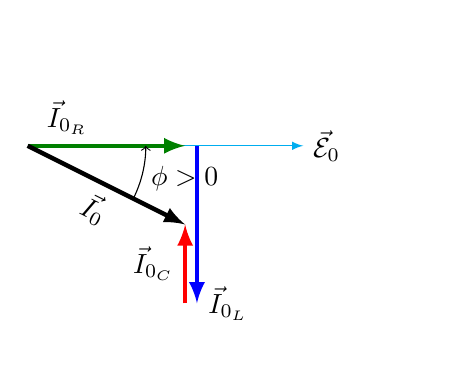
\begin{tikzpicture}[
				declare function = {
						IC = 1;
						IL = 2;
						IR = 2;
						DLC = (IL - IC);
						PhI = -atan(DLC/IR);
					},
			]
			\path[use as bounding box] (0,1.5) rectangle ++(5,-4);
			\draw[-latex, cyan] (0,0) -- ++(3.5,0) node[right, color=black] {$\vec{\mathcal{E}}_0$};
			\draw[-latex,  green!50!black,ultra thick] (0,0) -- ++(IR,0) node[above, pos=0.25, color=black] {$\vec{I}_{0_R}$};
			\draw[-latex,  blue, ultra thick] (IR+0.15,0) -- ++(0,-IL) node[right, color=black] {$\vec{I}_{0_L}$};
			\draw[-latex,  red, ultra thick] (IR,-IL) -- ++(0,IC) node[left, color=black, pos=0.5] {$\vec{I}_{0_C}$};
			\draw[-latex,  black, ultra thick] (0,0) -- (PhI:{IR/cos(PhI)}) node[below, color=black, pos=0.5, sloped] {$\vec{I}_{0}$} coordinate (I);
			\draw[<-] (0,0) ++(1.5,0) arc(0:PhI:1.5) node[pos=0.6, right] {$\phi > 0$};
		\end{tikzpicture}
		\caption{$\omega < \omega_0$}
		\label{pic:P-vector_diagrams<}
	\end{subfigure}
	\begin{subfigure}[b]{0.30\linewidth}
		\centering
		\begin{tikzpicture}[
				declare function = {
						IC = 1.5;
						IL = 1.5;
						IR = 2;
						DLC = (IL - IC);
						PhI = -atan(DLC/IR);
					},
			]
			\path[use as bounding box] (0,1.5) rectangle ++(5,-4);
			\draw[-latex, cyan] (0,0) -- ++(3.5,0) node[right, color=black] {$\vec{\mathcal{E}}_0$};
			\draw[-latex,  green!50!black,ultra thick] (0,0) -- ++(IR,0) node[above, pos=0.5, color=black] {$\vec{I}_{0_R} = \vec{I}_{0}$};
			\draw[-latex,  blue, ultra thick] (IR+0.15,0) -- ++(0,-IL) node[right, color=black] {$\vec{I}_{0_L}$};
			\draw[-latex,  red, ultra thick] (IR,-IL) -- ++(0,IC) node[left, color=black, pos=0.2] {$\vec{I}_{0_C}$};
		\end{tikzpicture}
		\caption{$\omega = \omega_0$}
		\label{pic:P-vector_diagrams=}
	\end{subfigure}
	\begin{subfigure}[b]{0.30\linewidth}
		\centering
		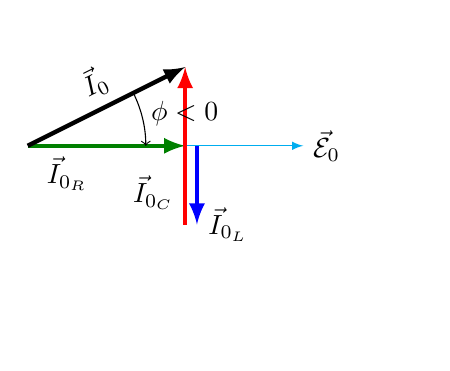
\begin{tikzpicture}[
				declare function = {
						IC = 2;
						IL = 1;
						IR = 2;
						DLC = (IL - IC);
						PhI = -atan(DLC/IR);
					},
			]
			\path[use as bounding box] (0,1.5) rectangle ++(5,-4);
			\draw[-latex, cyan] (0,0) -- ++(3.5,0) node[right, color=black] {$\vec{\mathcal{E}}_0$};
			\draw[-latex,  green!50!black,ultra thick] (0,0) -- ++(IR,0) node[below, pos=0.25, color=black] {$\vec{I}_{0_R}$};
			\draw[-latex,  blue, ultra thick] (IR+0.15,0) -- ++(0,-IL) node[right, color=black] {$\vec{I}_{0_L}$};
			\draw[-latex,  red, ultra thick] (IR,-IL) -- ++(0,IC) node[left, color=black, pos=0.2] {$\vec{I}_{0_C}$};
			\draw[-latex,  black, ultra thick] (0,0) -- (PhI:{IR/cos(PhI)}) node[above, color=black, pos=0.5, sloped] {$\vec{I}_{0}$} coordinate (I);
			\draw[<-] (0,0) ++(1.5,0) arc(0:PhI:1.5) node[pos=0.6, right] {$\phi < 0$};
		\end{tikzpicture}
		\caption{$\omega > \omega_0$}
		\label{pic:P-vector_diagrams>}
	\end{subfigure}
\caption{Векторна діаграма для паралельно контура}
\label{pic:P-vector_diagrams}
\end{figure}
%---------------------------------------------------------
\end{enumerate}

%\subsection{Вимірювання фазового зсуву}
%
%Для вимірювання фазових співвідношень можна використовувати двоканальний осцилограф. Наприклад, необхідно  виміряти зсув фаз між двома напругами $U_x$ та $U_y$ однакової частоти. Подамо ці напруги на горизонтальну і вертикальну розгортки осцилографа:
%\begin{align}
%    U_x &= U_{0x}\cos\omega t, \\
%    U_y &= U_{0y}\cos(\omega t + \phi),
%\end{align}
%де $U_{0x}$ та $U_{0y}$ амплітуди цих наруг, $\phi$~--- зсув фаз між ними. Виключивши час $t$ з цих рівнянь, отримаємо рівняння кривої, яка називається \href{https://uk.wikipedia.org/wiki/Фігури\_Ліссажу}{фігурою Ліссажу}:
%\begin{equation}\label{eq:Lissajous}
%    \frac{U_x^2}{U_{0x}^2} + \frac{U_y^2}{U_{0y}^2} - 2\frac{U_xU_y}{U_{0x}U_{0y}}\cos\phi = \sin^2\phi.
%\end{equation}
%Оскільки частоти коливань однакові, то фігурою Ліссажу є еліпс (або коло та пряма, в залежності від зсуву фаз $\phi$), саме така крива і буде спостерігатись на екрані осцилографа~\ref{fig:Lissajous}:
%
%\begin{wrapfigure}{l}{0.6\linewidth}\centering
%    % !TeX program = lualatex
% !TeX encoding = utf8
% !TeX spellcheck = uk_UA
% !TeX root =../LabWork.tex

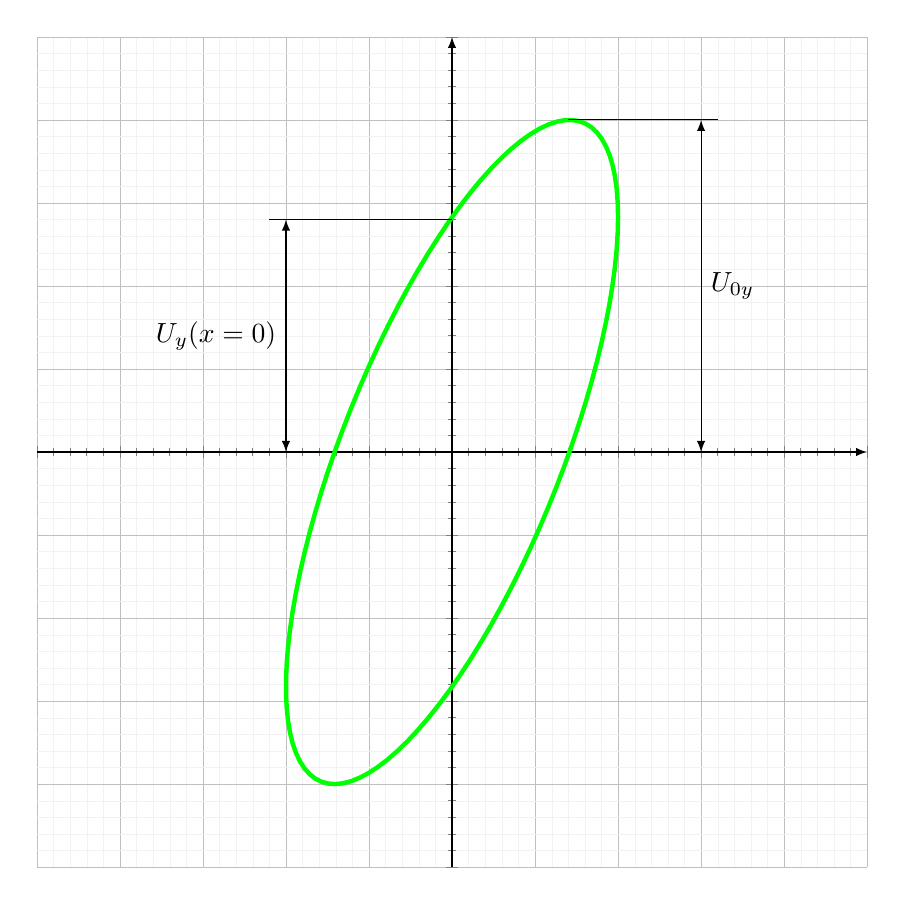
\begin{tikzpicture}

\begin{axis}[%
% === Налаштування сітки ===
axis lines = middle,
axis line style={-latex, black},
grid=both,
grid style={line width=.1pt, draw=gray!10},
major grid style={line width=.2pt,draw=gray!50},
minor tick num=4,
width=1\linewidth,
height=1\linewidth,
% === Вибір підписів шкали для відображення ===
xticklabel=\empty,
yticklabel=\empty,
xmin = -5,
xmax = 5,
ymin = -5,
ymax = 5,
trig format plots=rad,
]

\addplot[samples=100, mark=none, green, ultra thick, domain=0:2*pi,] ({2*cos(x)}, {4*cos(x  + pi/4)});
\draw[latex-latex] (axis cs:3,0) -- node[right] {$U_{0y}$ } (axis cs:3,4);
\draw[] (axis cs:1.4,4) -- (axis cs:3.2,4);

\draw[latex-latex] (axis cs:-2,0) -- node[left] {$U_{y}(x=0)$ } (axis cs:-2,2.8);
\draw[] (axis cs:0,2.8) -- (axis cs:-2.2,2.8);
\end{axis}
\end{tikzpicture}%
%\caption{Еліпс на екрані осцилографа}
%\label{fig:Lissajous}
%\end{wrapfigure}
%Орієнтація еліпса відносно координатних осей $X$ і $Y$ залежить як від шуканого фазового зсуву $\phi$ (за умови, що підсилення каналів однакове). При $\phi = 0$ еліпс вироджується в пряму, що перетинає квадранти I та III картинки на осцилографі. При збільшенні і при зменшенні $\phi$ еліпс стає більш-менш <<повним>>, але його велика піввісь продовжує перетинати перший і третій квадранти.
%
%Для вимірювання зсуву фаз між напругами  $U_x$ та $U_y$ можна вимірювати <<повноту>> еліпса, викорисовуючи наступну процедуру наступний прийом (рис.~\ref{fig:Lissajous}): знайдемо за картиною з осцілографу значення $U_{0y}$ та $U_y(x=0)$  і підставимо в рівняння~\eqref{eq:Lissajous}, отримаємо:
%\[
%       \frac{U_y^2(x=0)}{U_{0y}^2} = \sin^2\phi,
%\] 
%тобто, зсув фаз буде визначатись як:
%\[
%    \phi = \pm \arcsin\left( \frac{U_y^2(x=0)}{U_{0y}^2}\right).
%\]


\begin{More}

	Метод векторних діаграм і метод комплексних амплітуд --- методи опису синусоїдальних коливань, які мають свої переваги і недоліки
	\begin{enumerate}[label=$\checkmark$]
		\item Метод комплексних амплітуд більш потужний, оскільки природно включає в себе, складання і розв'язки систем рівнянь будь-якої складності, наприклад, для розгалужених кіл змінного струму, в той час як метод векторних діаграм в чистому вигляді все ж обмежений задачами, які передбачають графічні розрахунки.
		\item Метод векторних діаграм є більш наочним, а отже в деяких випадках потенційно більш надійний (дозволяє до певної міри уникнути грубих випадкових помилок, які можуть зустрічатися при абстрактних алгебраїчних обчисленнях) і дозволяє в деяких випадках досягти в якомусь сенсі більш глибокого розуміння задачі.
	\end{enumerate}
\end{More}

% !TeX program = lualatex
% !TeX encoding = utf8
% !TeX spellcheck = uk_UA
% !TeX root =../LabWork.tex

\section{Резонанс напруг у послідовному \boldmath{$RLC$}-колі}

Використовуючи~\eqref{CI0_phase} та \eqref{eq:U}, модулі амплітудних значень напруг на елементах послідовного $RLC$-кола можна записати у вигляді:
\begin{align}
	U_{0_R} & = I_0R =   \frac{\mathcal{E}_0 R}{\sqrt{R^2  +   \left(  \omega L - \frac{1}{\omega C} \right)^2}}, \label{U0R}       \\
	U_{0_L} & = I_0X_L = \frac{\mathcal{E}_0 \omega L}{\sqrt{R^2  +   \left(  \omega L - \frac{1}{\omega C} \right)^2}} \label{U0L} \\
	U_{0_C} & = I_0X_C = \frac{\mathcal{E}_0}{\omega C\sqrt{R^2  +   \left(  \omega L - \frac{1}{\omega C} \right)^2}}\label{U0C}.
\end{align}
Ці формули дозволяють зобразити графічно залежність амплітуд коливань напруг  від частоти генератора~\ref{plt:S-AFC} і носять назву амплітудно-частотних характеристик (АЧХ), або резонансних кривих. 

%---------------------------------------------------------
\begin{figure}[!h]\centering
	\begin{minipage}{0.75\linewidth}
		% !TeX program = lualatex
% !TeX encoding = utf8
% !TeX spellcheck = uk_UA
% !TeX root =../LabWork.tex

\begin{tikzpicture}%
[
declare function ={
L = 2;
C = 0.5;
R = 0.9;
U=15;
omegares = 1/sqrt(L*C);
Q = 1/R*sqrt(L/C);
UC(\x) = U/(x*C)/sqrt(R^2 + (x*L-1/(C*x))^2);
UL(\x) = U*(x*L)/sqrt(R^2 + (x*L-1/(C*x))^2);
UR(\x) = U*R/sqrt(R^2 + (x*L-1/(C*x))^2);
phi(\x) = rad(atan((x*L-1/(x*C))/R));
}
]
			\begin{groupplot}[group style={group size=1 by 2, vertical sep=2cm}]
				%---------------------------------------------------------
				\nextgroupplot[title={\small Амплітудно-частотна характеристики напруг},
					% === Налаштування сітки ===
					grid = both,
					major grid style={line width=.2pt,draw=gray!50},
					minor tick num = 4,
					minor grid style = {line width=.1pt,draw=gray!10},
					% === Налаштування положення координатних осей ===
					%axis x line=center, % top, center, bottom
					%axis y line=center, % left, center, right
					axis lines = middle,
					axis line style={-stealth},
					% === Підпис координатних осей ===
					xlabel={$\omega$},
					ylabel={$U$},
					extra x ticks={omegares},
					extra x tick labels={$\omega_0$},
					xticklabels={},
					yticklabels={},
					extra y ticks={U, Q*U},
					extra y tick labels={$\mathcal{E}_0$, $Q \mathcal{E}_0$},
					% === Положення підпису координатних осей ===
					xlabel style={below right},
					ylabel style={above left},
					xtick style={draw=none},
					ytick style={draw=none},
					% === Вибір підписів шкали для відображення ===
					xtick = {},
					ytick = {},
					% === Налаштування мінімальних та максимальних значень координат ===
					xmin = 0,
					xmax =  2*omegares,
					ymin = 0,
					ymax =  40,
					% === Налаштування розміру графіка ===
					width=1\linewidth,
					height=0.75\linewidth,
					]
				\addplot [ultra thick, samples = 1000, red, thick, domain=0.001:2*omegares] {UC(x)};
				\addplot [ultra thick,samples = 1000, blue, thick, domain=0.001:2*omegares] {UL(x)};
				\addplot [ultra thick,samples = 1000, green!50!black, thick, domain=0.001:2*omegares] {UR(x)};
				\legend{$U_{0_C}$,$U_{0_L}$,$U_{0_R}$}
				%---------------------------------------------------------
				\nextgroupplot[title={\small Фазово-частотна характеристика послідовного кола},
					% === Налаштування сітки ===
					grid = both,
					major grid style={line width=.2pt,draw=gray!50},
					minor tick num = 4,
					minor grid style = {line width=.1pt,draw=gray!10},
					% === Налаштування положення координатних осей ===
					axis lines = middle,
					yticklabel pos=right,
					axis line style={-stealth},
					% === Підпис координатних осей ===
					xlabel={$\omega$},
					ylabel={$\phi$},
					xticklabels={},
					yticklabels={},
					extra tick style={% changes for all extra ticks
							tick align=outside,
							grid style={dashed,draw=black}
						},
%					extra y tick style={
%	
%						},
					extra x ticks = {omegares},
					extra x tick labels={$\omega_0$},
					extra y ticks = {-pi/2,pi/2},
					ytick = {-pi/2,-pi/4,0,pi/4,pi/2},
					extra y tick labels={$-\frac{\pi}{2}$,$\frac{\pi}{2}$},
					xtick style={draw=none},
					ytick style={draw=none},
					% === Положення підпису координатних осей ===
					xlabel style={below right},
					ylabel style={above right},
					% === Налаштування мінімальних та максимальних значень координат ===
					xmin = 0,
					xmax =  2*omegares,
					ymin = -pi/2,
					ymax =  pi/2,
					% === Налаштування розміру графіка ===
					width=1\linewidth,
					height=0.4\linewidth,
				]
				\addplot [ultra thick,samples = 1000, green!50!black, thick, domain=0.01:2*omegares, name path global=ResCurve] {phi(x)};
				%---------------------------------------------------------
			\end{groupplot}
		\end{tikzpicture}
		\caption{Амплітудно- і фазовочастотні характеристики послідовного кола}
		\label{plt:S-AFC}
	\end{minipage}
\end{figure}
%---------------------------------------------------------


%\begin{figure}[h!]\centering
%    % !TeX program = lualatex
% !TeX encoding = utf8
% !TeX spellcheck = uk_UA
% !TeX root =../LabWork.tex

	\begin{subfigure}[b]{0.30\linewidth}
		\centering
		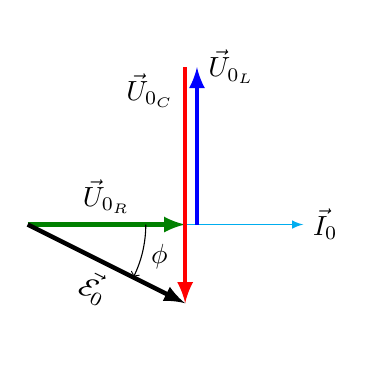
\begin{tikzpicture}[
				declare function = {
						UC = 3;
						UL = 2;
						UR = 2;
						DLC = (UL - UC);
						PhU = atan (DLC/UR);
					},
			]
			\path[use as bounding box] (0,-1.5) rectangle ++(4,4);
			\draw[-latex, cyan] (0,0) -- ++(3.5,0) node[right, color=black] {$\vec{I}_0$};
			\draw[-latex,  green!50!black,ultra thick] (0,0) -- ++(UR,0) node[above, pos=0.5, color=black] {$\vec{U}_{0_R}$};
			\draw[-latex,  blue, ultra thick] (UR+0.15,0) -- ++(0,UL) node[right, color=black] {$\vec{U}_{0_L}$};
			\draw[-latex,  red, ultra thick] (UR,UL) -- ++(0,-UC) node[left, color=black, pos=0.1] {$\vec{U}_{0_C}$};
			\draw[-latex,  black, ultra thick] (0,0) -- (PhU:{UR/cos(PhU)}) node[below, color=black, pos=0.5, sloped] {$\vec{\mathcal{E}}_{0}$} coordinate (U);
			%	\draw[dashed] (\UR,0) -- (U) (0,\DLC) -- (U);
			\draw[->] (0,0) ++(1.5,0) arc(0:PhU:1.5) node[pos=0.6, right] {$\phi$};
		\end{tikzpicture}
		\caption{$\omega < \omega_0$}
		\label{pic:S-vector_diagrams<}
	\end{subfigure}
	\begin{subfigure}[b]{0.30\linewidth}
		\centering
		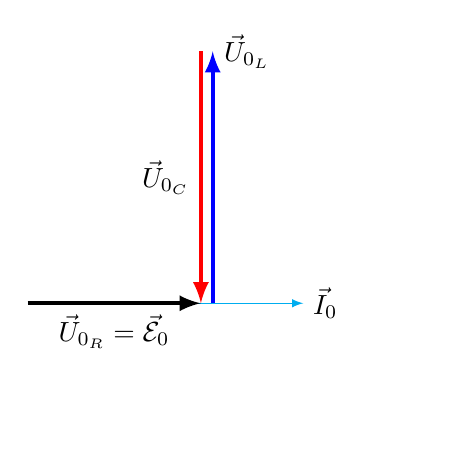
\begin{tikzpicture}[
				declare function = {
						UC = 3.2;
						UL = 3.2;
						UR = 2.2;
						DLC = (UL - UC);
						PhU = atan (DLC/UR);
					},
			]
			\path[use as bounding box] (0,-1.5) rectangle ++(5,5);
			\draw[-latex, cyan] (0,0) -- ++(3.5,0) node[right, color=black] {$\vec{I}_0$};
			\draw[-latex,  black,ultra thick] (0,0) -- ++({2/cos(atan(1/2.2)},0) node[below, pos=0.5, color=black] {$\vec{U}_{0_R} = \vec{\mathcal{E}}_{0}$};
			\draw[-latex,  blue, ultra thick] (UR+0.15,0) -- ++(0,UL) node[right, color=black] {$\vec{U}_{0_L}$};
			\draw[-latex,  red, ultra thick] (UR,UL) -- ++(0,-UC) node[left, color=black, pos=0.5] {$\vec{U}_{0_C}$};
		\end{tikzpicture}
		\caption{$\omega = \omega_0$}
		\label{pic:S-vector_diagrams=}
	\end{subfigure}
	\begin{subfigure}[b]{0.30\linewidth}
		\centering
		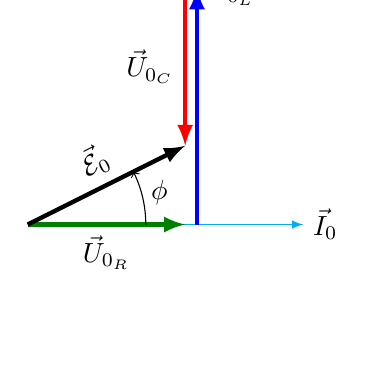
\begin{tikzpicture}[
				declare function = {
						UC = 2;
						UL = 3;
						UR = 2;
						DLC = (UL - UC);
						PhU = atan (DLC/UR);
					},
			]
			\path[use as bounding box] (0,-1.5) rectangle ++(4,4);
			\draw[-latex, cyan] (0,0) -- ++(3.5,0) node[right, color=black] {$\vec{I}_0$};
			\draw[-latex,  green!50!black,ultra thick] (0,0) -- ++(UR,0) node[below, pos=0.5, color=black] {$\vec{U}_{0_R}$};
			\draw[-latex,  blue, ultra thick] (UR+0.15,0) -- ++(0,UL) node[right, color=black] {$\vec{U}_{0_L}$};
			\draw[-latex,  red, ultra thick] (UR,UL) -- ++(0,-UC) node[left, color=black, pos=0.5] {$\vec{U}_{0_C}$};
			\draw[-latex,  black, ultra thick] (0,0) -- (PhU:{UR/cos(PhU)}) node[above, color=black, pos=0.5, sloped] {$\vec{\mathcal{E}}_{0}$} coordinate (U);
			%	\draw[dashed] (\UR,0) -- (U) (0,\DLC) -- (U);
			\draw[->] (0,0) ++(1.5,0) arc(0:PhU:1.5) node[pos=0.6, right] {$\phi$};
		\end{tikzpicture}
		\caption{$\omega > \omega_0$}
		\label{pic:S-vector_diagrams>}
	\end{subfigure}
%	\caption{Векторні діаграми напруг для послідовного кола. \\ {\small \itshape Зсув фаз $\phi$ прийнято позначати стрілкою, яка напрямлена від вектора струму до вектора напруги}}
%	\label{pic:S-vector_diagrams}
%\end{figure}

З формули~\eqref{CI0} видно, що за умови коли частота генератора співпаде з власною частотою контура $\omega = \omega_0 = \frac{1}{\sqrt{LC}}$, реактивні опори котушки і конденсатора стануть однаковими:
\begin{equation}
	\omega L = \frac{1}{\omega C},
\end{equation}
а амплітуда сили струму в послідовному $RLC$-колі досягає свого максимального значення $I_0 = \dfrac{\mathcal{E}_0}{R}$ як і напруга на резисторі, яка дорівнює амплітудному значенню напруги на генераторі $\mathcal{E}_0$. Напруги на конденсаторі і котушці при цьому приймають однакові значення (див. формули~\eqref{U0R} -- \eqref{U0L}):
\begin{align}\label{ULC}
	U_{0_R}    & = \mathcal{E}_0                                                             \\
	U_{0_C}    & = U_{0_L} = \frac{1}{R} \sqrt{\frac{L}{C}} \mathcal{E}_0 = Q \mathcal{E}_0, \label{eq:Q}\\
	U_{0_{LC}} & = U_{0_L} - U_{0_C} = 0 
\end{align}
де $U_{0_{LC}}$~--- амплітуда напруги на $LC$-ділянці. Також слід відмітити, що амплітуди напруги на конденсаторі та котушці індуктивності перевищують напругу на генераторі у $Q$  разів (див.~\eqref{eq:Q}), де

\begin{equation}\label{eq:Qdef}
    Q = \frac{1}{R}\sqrt{\frac{L}{C}}.
\end{equation}
Величина $Q$ називається \href{http://femto.com.ua/articles/part_1/1110.html}{\emph{добротністю контуру}}, її значення завжди більше одиниці (рис.~\ref{plt:S-AFC}). Отже, явище перевищення амплітуд напруг на конденсаторі та котушці в $Q$ разів порівнянні з амплітудою напруги на генераторі в послідовному контурі при співпадінні частоти генератора і власної частоти кола називається \emph{резонансом напруг}. 

%\noindent\bigskip%
%\begin{More}
%
%	З фізичної точки зору, при явищі резонансу напруг в колі відбувається обмін енергією між магнітним полем котушки і електричним полем конденсатора, при такому обміні енергією між полем і джерелом живлення не відбувається.
%\end{More}

\subsection{Енергетичні процеси в послідовному $RLC$-колі}

Фізичний сенс добротності можна побачити, якщо перейти до аналізу енергетичних процесів в коливальному контурі. Розглянемо середню потужність, яка розсіюється контуром у вигляді теплоти за період:
\begin{equation}\label{eq:Power}
    P = \frac12 I_0^2R = \frac12 \frac{\mathcal{E}_0^2R}{R^2 + \left(\omega L - \frac{1}{\omega C}\right)^2} = \frac{\mathcal{E}_0^2}{2R}\, \frac{1}{1  + \left(\omega^2 - \omega_0^2\right)^2 L^2/(R\omega^2)},
\end{equation}
де $I_0$~--- амплітуда коливань струму. Крива, яка описується формулою~\eqref{eq:Power}
 має вигляд, зображений на рис.~\ref{plt:P(o)}.

%---------------------------------------------------------
\begin{center}%[!htbp]\centering
		% !TeX program = lualatex
% !TeX encoding = utf8
% !TeX spellcheck = uk_UA
% !TeX root =../LabWork.tex

		\begin{tikzpicture}
			\pgfset{fpu=true}
			\pgfmathsetmacro{\L}{2e-3}
			\pgfmathsetmacro{\C}{2.2e-6}
			\pgfmathsetmacro{\R}{10}
			\pgfmathsetmacro{\RL}{0.8}
			\pgfmathsetmacro{\Ri}{5}
			\pgfmathsetmacro{\U}{5}
			\pgfmathsetmacro{\omegares}{1/sqrt(\L*\C)}
			\pgfmathsetmacro{\Q}{sqrt(\L/\C)/\RL}
			\pgfmathsetmacro{\Imax}{\U/(\R + \Ri + \RL)}
			\pgfset{fpu=false}
			\begin{axis}[clip = false,
					% === Налаштування сітки ===
					grid = both,
					grid style={line width=.1pt, draw=gray!10},
					major grid style={line width=.2pt,draw=gray!50},
					minor tick num = 5,
					minor grid style = {line width=.1pt,draw=gray!10},
					% === Налаштування положення координатних осей ===
					%axis x line=center, % top, center, bottom
					%axis y line=center, % left, center, right
					axis lines = middle,
					axis line style={-stealth},
					% === Підпис координатних осей ===
					xticklabels={},
					%xlabel={$\omega$},
					ylabel={$\frac{P}{P_{\max}}$},
					xtick scale label code/.code={$\omega$},
					yticklabels={},
					xtick style={draw=none},
					ytick style={draw=none},
					% === Положення підпису координатних осей ===
					%				xlabel style={below right},
					ylabel style={above right},
					every x tick scale label/.style={at={(1,0)}, anchor = north},
					extra y ticks={1/2, 1},
					extra x ticks={\omegares},
					extra y tick labels={$\frac12$, $1$},
					extra x tick labels={$\omega_0$},
					% === Вибір підписів шкали для відображення ===
					xtick = {},
					ytick = {},
					% === Налаштування мінімальних та максимальних значень координат ===
					xmin = 0,
					xmax =  2*\omegares,
					ymin = 0,
					ymax =  1,
					% === Налаштування розміру графіка ===
					width=1\linewidth,
					height=1\linewidth,
				]
				\addplot [ultra thick,samples = 500, green!50!black, thick, domain=0.5*\omegares:2*\omegares, name path global=ResCurve] {(\R + \RL + \Ri)^2/((\R + \RL + \Ri)^2 + (x*\L-1/(\C*x))^2)};

				\path[name path=line] (axis cs:0, {1/2}) -- (axis cs:3*\omegares,{1/2});
				\draw [thick,
					dashed,
					name intersections={of=ResCurve and line},
				] (axis cs:0, {1/2}) -- (intersection-1) -- (intersection-2) (intersection-1) -- (intersection-1 |-0,0) node [below left] {$\omega_0 - \Delta\omega$} (intersection-2) -- (intersection-2 |-0,0) node [below right] {$\omega_0 + \Delta\omega$};
				\fill [white, draw=green!50!black, name intersections={of=ResCurve and line}] (intersection-1) circle (0.1cm) (intersection-2) circle (0.1cm);
			\end{axis}
		\end{tikzpicture}
		\captionof{figure}{Резонансна крива потужності, що розсіюється на резисторі в послідовному контурі}
		\label{plt:P(o)}
\end{center}
%---------------------------------------------------------

При резонансі потужність досягає максимального значення $P_{\max} = \frac12\frac{\mathcal{E}_0^2}{R}$. З фізичної точки зору, це означає, що вся енергія, яка підводиться до кола розсіюється на резисторі, а енергія, яка була запасена в  конденсаторі та котушці індуктивності у вигляді електромагнітного поля, циркулює між цими цими елементами, тобто обмін енергією між полем і джерелом живлення не відбувається.  Ця ситуація виглядає так, ніби зовнішня напруга прикладена лише до резистора. Якщо контур мало поглинає, а більше запасає енергії, то потужність, що розсіюється помітна лише поблизу резонансу на частоті $\omega_0$ і в формул~\eqref{eq:Power} можна скористатись наближенням:
\[
    \omega^2 - \omega_0^2 \approx 2\omega_0\Delta\omega, 
\]
і переписати \eqref{eq:Power} у вигляді:
\begin{equation}\label{eq:Power2}
    P =  \frac{\mathcal{E}_0^2}{2R}\, \frac{1}{1  + (\Delta\omega)^2\tau^2 },
\end{equation}
де $\tau = 2L/R$. З цієї формули видно, що потужність, вдвічі меншу за максимальну можна знайти, якщо  в знаменнику покласти $(\Delta\omega)^2\tau^2 = 1$, тобто коли $\Delta\omega = \frac{R}{2L}$. Величина $\Delta\omega$ називається півшириною резонансної кривої (в радіотехніці вона називається смугою пропускання). Оскільки добротність визначається формулою~\eqref{eq:Qdef}, то легко бачити, що з іншого боку, її можна знайти як
\begin{equation*}
    Q = \frac{1}{R}\sqrt{\frac{L}{C}} = \frac{\omega_0 L}{R} = \frac{\omega_0}{2\Delta\omega},
\end{equation*}
тобто як  відношення резонансної частоти до ширини резонансної кривої потужності. Звідки, зрозуміла назва <<добротність>>, яка означає, що контур тим якісніше (добротніше) чим менше розсіюється в ньому енергії енергії, або чим більше її накопичується за період. Більш високе значення цього показника відповідає більш вузькій кривій, а у випадку ідеального кола ($R = 0$) його добротність нескінченна.

\subsection{Експериментальний метод визначення добротності}

Аналіз резонансної кривої потужності підказує експериментальний спосіб визначення добротності. Ми будемо розглядати в якості резонансної кривої залежність напруги на резисторі як функцію частоти генератора $U_{0R} = f(\omega)$, або  залежність струму в контурі від тієї ж змінної $I = f(\omega)$ (це не суттєво, оскільки ці величини відрізняються лише множником $R$), а ширину кривої $2\Delta\omega$ визначати на $\dfrac1{\sqrt2}\approx 0.707$ від висоти максимуму (рис.~\ref{plt:I(o)}),  оскільки потужність і енергія пропорційні квадрату амплітуди коливань $P \sim I_0^2 \sim U_0^2 $, то рівню $0.707$ відповідає точка половинної потужності, тобто $(0.707)^2 = 0.5$, а добротність також можна визначити за формулою 
\begin{equation*}
Q = \frac{\omega_0}{2\Delta\omega}
\end{equation*}
з урахуванням вищесказаного.

%---------------------------------------------------------
\begin{figure}[!h]\centering
	\begin{minipage}{0.75\linewidth}
		% !TeX program = lualatex
% !TeX encoding = utf8
% !TeX spellcheck = uk_UA
% !TeX root =../LabWork.tex

		\begin{tikzpicture}
			\pgfset{fpu=true}
			\pgfmathsetmacro{\L}{2e-3}
			\pgfmathsetmacro{\C}{2.2e-6}
			\pgfmathsetmacro{\R}{10}
			\pgfmathsetmacro{\RL}{0.8}
			\pgfmathsetmacro{\Ri}{5}
			\pgfmathsetmacro{\U}{5}
			\pgfmathsetmacro{\omegares}{1/sqrt(\L*\C)}
			\pgfmathsetmacro{\Q}{sqrt(\L/\C)/\RL}
			\pgfmathsetmacro{\Imax}{\U/(\R + \Ri + \RL)}
			\pgfset{fpu=false}
			\begin{axis}[clip = false,
					% === Налаштування сітки ===
					grid = both,
					grid style={line width=.1pt, draw=gray!10},
					major grid style={line width=.2pt,draw=gray!50},
					minor tick num = 5,
					minor grid style = {line width=.1pt,draw=gray!10},
					% === Налаштування положення координатних осей ===
					%axis x line=center, % top, center, bottom
					%axis y line=center, % left, center, right
					axis lines = middle,
					axis line style={-stealth},
					% === Підпис координатних осей ===
					xticklabels={},
					%xlabel={$\omega$},
					ylabel={$\frac{I_{0}}{I_{\max}}$},
					xtick scale label code/.code={$\omega$},
					yticklabels={},
					xtick style={draw=none},
					ytick style={draw=none},
					% === Положення підпису координатних осей ===
					%				xlabel style={below right},
					ylabel style={above right},
					every x tick scale label/.style={at={(1,0)}, anchor = north},
					extra y ticks={1/sqrt(2), 1},
					extra x ticks={\omegares},
					extra y tick labels={$\frac{1}{\sqrt2}$, $1$},
					extra x tick labels={$\omega_0$},
					% === Вибір підписів шкали для відображення ===
					xtick = {},
					ytick = {},
					% === Налаштування мінімальних та максимальних значень координат ===
					xmin = 0,
					xmax =  3*\omegares,
					ymin = 0,
					ymax =  1,
					% === Налаштування розміру графіка ===
					width=1\linewidth,
					height=1\linewidth,
				]
				\addplot [ultra thick,samples = 500, green!50!black, thick, domain=0.1*\omegares:3*\omegares, name path global=ResCurve] {(\R + \RL + \Ri)/sqrt((\R + \RL + \Ri)^2 + (x*\L-1/(\C*x))^2)};

				\path[name path=line] (axis cs:0, {1/sqrt(2)}) -- (axis cs:3*\omegares,{1/sqrt(2)});
				\draw [thick,
					dashed,
					name intersections={of=ResCurve and line},
				] (axis cs:0, {1/sqrt(2)}) -- (intersection-1) -- (intersection-2) (intersection-1) -- (intersection-1 |-0,0) node [below left] {$\omega_0 - \Delta\omega$} (intersection-2) -- (intersection-2 |-0,0) node [below right] {$\omega_0 + \Delta\omega$};
				\fill [white, draw=green!50!black, name intersections={of=ResCurve and line}] (intersection-1) circle (0.1cm) (intersection-2) circle (0.1cm);
			\end{axis}
		\end{tikzpicture}
		\caption{Амплітудно-частотна характеристика напруги на резисторі послідовного контуру}
		\label{plt:I(o)}
	\end{minipage}
\end{figure}
%---------------------------------------------------------

Розглянемо тепер, як поводить себе модуль імпедансу всього контура, та модуль імпедансу $LC$-ділянки (рис.~\ref{plt:impedance_character}). З графіків видно, що за умови, коли частота генератора менше частоти резонансної частоти кола, ємнісний опір переважає над індуктивним і контур представляє для генератора опір ємнісного характеру. Якщо частота генератора більше резонансної частоти кола, то індуктивний опір більше ємнісного і контур для генератора є опором індуктивного характеру. При резонансі опір кола є суто активним.

%---------------------------------------------------------
\begin{figure}[!h]\centering
	% !TeX program = lualatex
% !TeX encoding = utf8
% !TeX spellcheck = uk_UA
% !TeX root =../LabWork.tex

	\begin{tikzpicture}[
			declare function={
					L  = 2;
					C  = 1.2e-3;
					R  = 80;
					omegares  = 1/sqrt(L*C);
					Q  = sqrt(L/C)/R;
					XL(\x) =\x*L;
					XC(\x) = 1/(C*\x) ;
				},
		]
		\begin{axis}[
				% === Налаштування сітки ===
				grid = both,
				major grid style={line width=.2pt,draw=gray!50},
				minor tick num = 4,
				minor grid style = {line width=.1pt,draw=gray!10},
				extra tick style={% changes for all extra ticks
						tick align=outside,
						grid style={dashed,draw=black}
					},
				extra x tick style={
						tick label style={
								xshift=5mm,
								/pgf/number format/.cd, fixed, fixed zerofill,
							}
					},
				% === Налаштування положення координатних осей ===
				axis lines = middle,
				axis line style={stealth-stealth},
				% === Підпис коор5динатних осей ===
				%				xticklabels={},
				xlabel={$\omega$},
				ylabel={},
				% === Положення підпису координатних осей ===
				ylabel style={above right},
				xticklabels={},
				yticklabels={},
				extra x ticks = {omegares},
				extra x tick labels = {$\omega_0$},
				ytick style={draw=none},
				xtick style={draw=none},
				% === Вибір підписів шкали для відображення ===
				xtick = {},
				ytick = {},
				legend style={at={(current axis.south east)},anchor=south east},
				% === Налаштування мінімальних та максимальних значень координат ===
				xmin = 6,
				xmax =  60,
				ymin = -150,
				ymax =  150,
				% === Налаштування розміру графіка ===
				width=1\linewidth,
				width=0.7\linewidth,
			]
			\addplot [ultra thick,samples = 500, blue, thick, domain=0.2*omegares:3*omegares,name path = UL]  {XL(x)};
			\addplot [ultra thick,samples = 500, red, thick, domain=0.2*omegares:3*omegares,name path = UC]  {-XC(x)};
			\addplot [ultra thick,samples = 500, green!50!black, thick, domain=0.2*omegares:3*omegares,name path = DU]  {XL(x)-XC(x)};
			\addplot [ultra thick,samples = 500, black, thick, domain=0.2*omegares:3*omegares,name path = DU]  {sqrt(R^2 + (XL(x)-XC(x))^2)};
			\legend{$X_L = \omega L$, $X_C = \frac{1}{\omega C}$, $Z_{LC} = X_L - X_C$, $Z = \sqrt{R^2 + (X_L - X_C)^2}$}
			\pgfplotsinvokeforeach{0.5,1,2}{
				\draw [-latex, blue, ultra thick] (axis cs:#1*omegares, 0) -- node[left] {$X_L$} (axis cs:#1*omegares, {XL(#1*omegares)});
				\draw [-latex, red, ultra thick] (axis cs:#1*omegares, 0) -- node[left] {$X_C$} (axis cs:#1*omegares, {-XC(#1*omegares)});
			}
			\draw [latex-latex, black] (axis cs:0.6*omegares, 0) -- node[fill=white] {$R$} (axis cs:0.6*omegares, {R});
			\draw [dashed] (axis cs:omegares, R) -- (axis cs:0.6*omegares, R);
		\end{axis}
	\end{tikzpicture}
	\caption{Характер зміни імпедансу кола}
	\label{plt:impedance_character}
\end{figure}

\noindent\bigskip%
\begin{More}

    В електротехніці резонанс напруг є небажаним явищем, оскільки він викликає перенапруження і вихід з ладу обладнання. Як простий приклад можна привести довгу кабельну лінію, яка з якоїсь причини виявилася не підключеною до навантаження, але при цьому живиться від проміжного трансформатора. Така лінія з розподіленою ємністю і індуктивністю, якщо її резонансна частота співпаде з частотою мережі живлення, просто буде пробита і вийде з ладу.

	Явище резонансу напруг використовують в \emph{електричних фільтрах}, наприклад якщо необхідно усунути з сигналу, що передається, складову струму певної частоти, то паралельно приймачу ставлять ланцюжок із сполучених послідовно конденсатора і котушки індуктивності, щоб струм резонансної частоти цього $LC$-ланцюжка замкнулося б через нього, і не потрапив до приймача. Тоді струми частоти далекою від резонансної частоти $LC$-ланцюжка будуть проходити в навантаження безперешкодно, і тільки близькі до резонансу по частоті струми --- знаходитимуть собі найкоротший шлях через $LC$-ланцюжок.

	Резонанс напруг широко застосовують в радіотехніці і використовують в тих випадках, коли потрібно посилити коливання напруги будь-якої визначеної частоти, при настроюванні радіоприймача на потрібну довжину хвилі. Вибірність приймача буде тим більшою, чим <<гостріша>> резонансна крива струму. Але уява про те, що під час радіоприймання потрібно, по можливості, збільшувати добротність контуру, бо при цьому збільшується напруга на конденсаторі, тобто чутливість приймача і усувається вплив сусідніх станцій, оскільки резонансна крива звужується, є помилкова, оскільки сигнал ніколи не буває ідеально монохроматичним. Тому, якщо крива резонансу надзвичайно вузька, то частина спектральних складових сигналу опиниться поза смугою пропускання контуру, що призведе до викривлення сигналу. Тому, наприклад, в телебаченні при передачі сигналів зображення використовується широка смуга частот 

\end{More}

\section{Резонанс струмів у паралельному $RLC$-колі}

Розглянемо електричне коло, де котушка, конденсатор та резистор з'єднані паралельно (рис.~\ref{pic:P-RLC}). В цьому випадку, напруга на кожному елементі буде однакова, а загальний струм $I$ буде дорівнювати сумі струмів, що протікають через кожний з елементів:
\begin{equation}
	I = I_R + I_C +I_L.
\end{equation}

В цьому випадку також можна скористатись методом комплексних амплітуд і визначити струми на окремих елементах контуру та загальний струм в колі:

\begin{align}
	I_R & = \frac{\mathcal{E}_0}{R} \cos(\omega t), \label{IR}                                                                     \\
	I_C & = \mathcal{E}_0\omega C \cos (\omega t + \frac{\pi}{2}), \label{IC}                                                      \\
	I_L & = \frac{\mathcal{E}_0}{\omega L}\cos (\omega t - \frac{\pi}{2}), \label{IL}                                              \\
	I   & = \mathcal{E}_0\sqrt{\frac{1}{R^2}  +   \left(  \omega C - \frac{1}{\omega L} \right)^2} \cos(\omega t + \phi).\label{I}
\end{align}

Зсув фаз $\phi$ між напругою та загальним струмом у колі дорівнюватиме:
\begin{equation}\label{P-phase_shift}
	\tg\phi = \frac{\omega C - \frac{1}{\omega L}}{R}.
\end{equation}

\begin{wrapfigure}[]{L}{0.4\linewidth}
	\begin{tikzpicture}[every circuit symbol/.style={thick}]
		\draw[thick] (0,-2) coordinate (START) to [ac source={rotate=-90,info={left:$\mathcal{E}_0$}}] (0,2) coordinate (AC) -- ++(2,0) coordinate (A) to [resistor={info'={$R$}}] ++(0,-4) coordinate (B) -- (START)
		(A) -- ++(1.5,0) coordinate (A1) to [capacitor={info'={$C$}}] ++(0,-4) coordinate (B1) -- (B)
		(A1) -- ++(1.5,0) coordinate (A2) to [inductor={info'={$L$}}] ++(0,-4) -- (B1)
		;
		\draw[->,red, thick] ([xshift=0.25cm]AC) -- node[color=black, above] {$I$} ++(1,0);
		\draw[->,red, thick] ([yshift=-0.25cm]A) -- node[color=black, left] {$I_R$} ++(0,-1);
		\draw[->,red, thick] ([yshift=-0.25cm]A1) -- node[color=black, left] {$I_C$} ++(0,-1);
		\draw[<-,red, thick] ([yshift=-0.25cm]A2) -- node[color=black, left] {$I_L$} ++(0,-1);
	\end{tikzpicture}
	\caption{Паралельне $RLC$-коло}
	\label{pic:P-RLC}
\end{wrapfigure}
З цих формул видно, що струм на резисторі $I_R$ коливається в фазі з напругою на генераторі, а його амплітуда не залежить від частоти, крім того, струми на конденсаторі $I_C$ і котушці $I_L$ коливаються в протифазі, і їх амплітуди залежать від частоти.

При частоті $\omega_0 = \dfrac{1}{\sqrt{CL}}$ амплітуда струму в колі досягає \emph{мінімального} значення $I_{0_{\min}} = I_{0_R}  = \dfrac{\mathcal{E}_0}{R}$, яка називається \emph{резонансною частотою}. При цьому струми на котушці та конденсаторі приймають однакові амплітудні значення $I_{0_C} = I_{0_L} = Q I_{0_{\min}}$, тобто перевищують силу струму в нерозгалудженій ділянці кола в $Q$ разів, при цьому контур поводить себе як активний опір ($\phi = 0$) величиною $Z = RQ^2$. Таке явище називається \emph{резонансом струмів} (рис.~\ref{plt:I(o)}).

%---------------------------------------------------------
\begin{figure}[!h]\centering
	% !TeX program = lualatex
% !TeX encoding = utf8
% !TeX spellcheck = uk_UA
% !TeX root =../LabWork.tex

	\begin{minipage}{0.75\linewidth}
		\begin{tikzpicture}[
			declare function = {
					L  = 2;
					C  = 0.5;
					R  = 10;
					RL  = 0.1;
					U = 2;
					omegares  = 1/sqrt(L*C);
					Q  = sqrt(L/C)/R;
					I(\x) = U*sqrt( (1/R + RL/(RL^2+\x^2*L^2))^2 + (\x*C-L*\x/(RL^2 + L^2*\x^2))^2 );				
				}
			]
			%---------------------------------------------------------
			\begin{groupplot}[group style={group size=1 by 2, vertical sep=2cm}]
				%---------------------------------------------------------
				\nextgroupplot[title={\small Амплітудно-частотна характеристика паралельного кола},
					% === Налаштування сітки ===
					grid = both,
					grid style={line width=.1pt, draw=gray!10},
					major grid style={line width=.2pt,draw=gray!50},
					minor tick num = 5,
					minor grid style = {line width=.1pt,draw=gray!10},
					% === Налаштування положення координатних осей ===
					%axis x line=center, % top, center, bottom
					%axis y line=center, % left, center, right
					axis lines = middle,
					axis line style={-stealth},
					% === Підпис координатних осей ===
					xlabel={$\omega$},
					ylabel={$I$},
					xticklabels={},yticklabels={},
					xtick style={draw=none},
					ytick style={draw=none},
					extra tick style={% changes for all extra ticks
							tick align=outside,
							major grid style={dashed,draw=black}
						},
					extra x ticks = {omegares},
					extra x tick labels={$\omega_0$},
					extra y ticks = {I(omegares),U*omegares*C},
					extra y tick labels={$I_0$, $I_0/Q$},
					% === Положення підпису координатних осей ===
					xlabel style={below right},
					ylabel style={above left},
					% === Вибір підписів шкали для відображення ===
					xtick = {},
					ytick = {},
					% === Налаштування мінімальних та максимальних значень координат ===
					xmin = 0,
					xmax =  2,
					ymin = 0,
					ymax =  4,
					% === Налаштування розміру графіка ===
					width=1\linewidth,
					height=0.96\linewidth,
				]
				\addplot [ultra thick,samples = 500, green!50!black, thick,domain=0:2, restrict y to domain=0:4, name path global=ResCurve] {I(x)};
				\addplot [ultra thick,samples = 500, red, thick, domain=0:2, restrict y to domain=0:4] {U*x*C};
				\addplot [ultra thick,samples = 500, blue, thick, domain=0:2, restrict y to domain=0:4] {U/sqrt(x^2*L^2 + RL^2)};
				\legend{$I_0$, $I_{0_C}$, $I_{0_L}$}
				%---------------------------------------------------------
				\nextgroupplot[title={\small Фазово-частотна характеристика паралельного кола},
					% === Налаштування сітки ===
					grid = both,
					grid style={line width=.1pt, draw=gray!10},
					major grid style={line width=.2pt,draw=gray!50},
					minor tick num = 4,
					minor grid style = {line width=.1pt,draw=gray!10},
					% === Налаштування положення координатних осей ===
					axis lines = middle,
					yticklabel pos=right,
					axis line style={-stealth},
					% === Підпис координатних осей ===
					xlabel={$\omega$},
					ylabel={$\phi$},
					xticklabels={},
					yticklabels={},
					extra tick style={% changes for all extra ticks
							tick align=outside,
							grid style={dashed,draw=black}
						},
%					extra y tick style={
%	
%						},
					extra x ticks = {omegares},
					extra x tick labels={$\omega_0$},
					extra y ticks = {-pi/2,pi/2},
					ytick = {-pi/2,-pi/4,0,pi/4,pi/2},
					extra y tick labels={$-\frac{\pi}{2}$,$\frac{\pi}{2}$},
					xtick style={draw=none},
					ytick style={draw=none},
					% === Положення підпису координатних осей ===
					xlabel style={below right},
					ylabel style={above right},
					% === Налаштування мінімальних та максимальних значень координат ===
					xmin = 0,
					xmax =  2*omegares,
					ymin = -pi/2,
					ymax =  pi/2,
					% === Налаштування розміру графіка ===
					width=1\linewidth,
					height=0.4\linewidth,
				]
				\addplot [ultra thick,samples = 1000, green!50!black, thick, domain=0.01:2*omegares, name path global=ResCurve] {rad(-atan((x*L-1/(x*C))/RL))};
				%---------------------------------------------------------
			\end{groupplot}
		\end{tikzpicture}
	\caption{Амплітудно- і фазовочастотні характеристики паралельного кола}
	\label{plt:P-AFC}
	\end{minipage}
\end{figure}
%---------------------------------------------------------

%\begin{figure}[h!]\centering
%            % !TeX program = lualatex
% !TeX encoding = utf8
% !TeX spellcheck = uk_UA
% !TeX root =../LabWork.tex

	\begin{subfigure}[b]{0.30\linewidth}
		\centering
		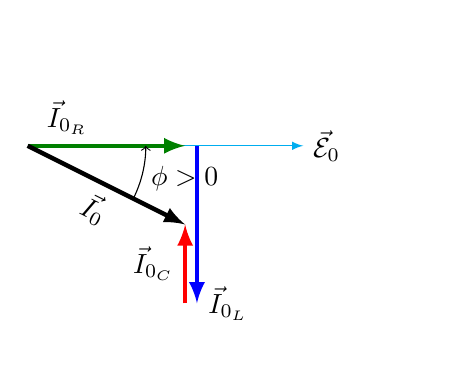
\begin{tikzpicture}[
				declare function = {
						IC = 1;
						IL = 2;
						IR = 2;
						DLC = (IL - IC);
						PhI = -atan(DLC/IR);
					},
			]
			\path[use as bounding box] (0,1.5) rectangle ++(5,-4);
			\draw[-latex, cyan] (0,0) -- ++(3.5,0) node[right, color=black] {$\vec{\mathcal{E}}_0$};
			\draw[-latex,  green!50!black,ultra thick] (0,0) -- ++(IR,0) node[above, pos=0.25, color=black] {$\vec{I}_{0_R}$};
			\draw[-latex,  blue, ultra thick] (IR+0.15,0) -- ++(0,-IL) node[right, color=black] {$\vec{I}_{0_L}$};
			\draw[-latex,  red, ultra thick] (IR,-IL) -- ++(0,IC) node[left, color=black, pos=0.5] {$\vec{I}_{0_C}$};
			\draw[-latex,  black, ultra thick] (0,0) -- (PhI:{IR/cos(PhI)}) node[below, color=black, pos=0.5, sloped] {$\vec{I}_{0}$} coordinate (I);
			\draw[<-] (0,0) ++(1.5,0) arc(0:PhI:1.5) node[pos=0.6, right] {$\phi > 0$};
		\end{tikzpicture}
		\caption{$\omega < \omega_0$}
		\label{pic:P-vector_diagrams<}
	\end{subfigure}
	\begin{subfigure}[b]{0.30\linewidth}
		\centering
		\begin{tikzpicture}[
				declare function = {
						IC = 1.5;
						IL = 1.5;
						IR = 2;
						DLC = (IL - IC);
						PhI = -atan(DLC/IR);
					},
			]
			\path[use as bounding box] (0,1.5) rectangle ++(5,-4);
			\draw[-latex, cyan] (0,0) -- ++(3.5,0) node[right, color=black] {$\vec{\mathcal{E}}_0$};
			\draw[-latex,  green!50!black,ultra thick] (0,0) -- ++(IR,0) node[above, pos=0.5, color=black] {$\vec{I}_{0_R} = \vec{I}_{0}$};
			\draw[-latex,  blue, ultra thick] (IR+0.15,0) -- ++(0,-IL) node[right, color=black] {$\vec{I}_{0_L}$};
			\draw[-latex,  red, ultra thick] (IR,-IL) -- ++(0,IC) node[left, color=black, pos=0.2] {$\vec{I}_{0_C}$};
		\end{tikzpicture}
		\caption{$\omega = \omega_0$}
		\label{pic:P-vector_diagrams=}
	\end{subfigure}
	\begin{subfigure}[b]{0.30\linewidth}
		\centering
		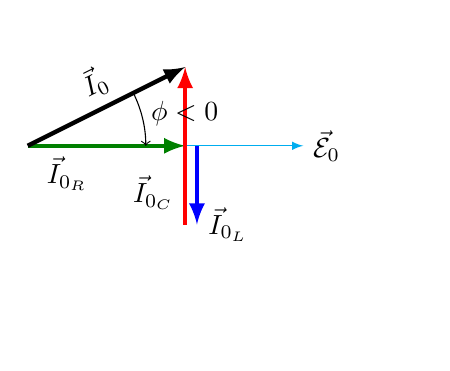
\begin{tikzpicture}[
				declare function = {
						IC = 2;
						IL = 1;
						IR = 2;
						DLC = (IL - IC);
						PhI = -atan(DLC/IR);
					},
			]
			\path[use as bounding box] (0,1.5) rectangle ++(5,-4);
			\draw[-latex, cyan] (0,0) -- ++(3.5,0) node[right, color=black] {$\vec{\mathcal{E}}_0$};
			\draw[-latex,  green!50!black,ultra thick] (0,0) -- ++(IR,0) node[below, pos=0.25, color=black] {$\vec{I}_{0_R}$};
			\draw[-latex,  blue, ultra thick] (IR+0.15,0) -- ++(0,-IL) node[right, color=black] {$\vec{I}_{0_L}$};
			\draw[-latex,  red, ultra thick] (IR,-IL) -- ++(0,IC) node[left, color=black, pos=0.2] {$\vec{I}_{0_C}$};
			\draw[-latex,  black, ultra thick] (0,0) -- (PhI:{IR/cos(PhI)}) node[above, color=black, pos=0.5, sloped] {$\vec{I}_{0}$} coordinate (I);
			\draw[<-] (0,0) ++(1.5,0) arc(0:PhI:1.5) node[pos=0.6, right] {$\phi < 0$};
		\end{tikzpicture}
		\caption{$\omega > \omega_0$}
		\label{pic:P-vector_diagrams>}
	\end{subfigure}
%	\caption{Векторні діаграми струмів для паралельного кола}
%	\label{pic:P-vector_diagrams}
%\end{figure}
%---------------------------------------------------------

При виникненні резонансу струму в колі його  реактивна складова стає рівною нулю, і як наслідок, повна провідність кола знижується до мінімального значення. Тому при постійній напрузі на затискачах даної схеми струм в нерозгалудженій частині  стає мінімальний, на відміну від резонансу напруги, коли струм максимальний. При цьому сумарний струм даному колі буде дорівнює векторній сумі всіх трьох струмів, два з яких (а саме $I_L$ і $I_C$) знаходяться в протифазі. Саме із-за того, що $I_L$ і $I_C$ знаходяться в протифазі в $LC$-ділянці починає протікати струм, який при резонансі може значно перевищувати сумарний струм $I$.

\noindent\bigskip%
\begin{More}

	Явище резонансу струмів використовується в прийомних пристроях для виділення електромагнітного сигналу в вузькому спектральному інтервалі частот поблизу резонансної частоти.

	В індукційних печах паралельно котушці, що створює змінне магнітне поле, підключають ємність. Якщо умови резонансу виконуються, то струм в котушці збільшується в багато разів, а струм в підвідних проводах при цьому відносно невеликий.
\end{More}







\part{Практична частина}
\labworklayout
\pagestyle{main}
\multiinclude{\Chapters}[]

\clearpage
\begin{refsection}
\nocite{Mat3, FLF6, AleshkevichElectro, Ledenev4, berkeley2}
\printbibliography[title={Рекомендована література}]
\end{refsection}

\end{document}